\section{Evaluation}
\subsection{Band Gap}
The raw data is plotted in figure \ref{fig:band_gap_raw_Ge} for 
germanium and \ref{fig:band_gap_raw_Si} for silicon. 
We set the $U-I$-converter to $15.03 \pm 0.03\,$mA for Ge 
and $0.75 \pm 0.01\,$mA for Si. The aperture was opened to 
$-10.0$--$+10.0\,$mm for both samples. Further settings 
not relevant for the evaluation, such as the settings of the gains, 
can be looked up in the 
handwritten records of the experiment in the appendix, 
\ref{sec:records_band_gap}. 
\begin{figure}
    \centering
    \begin{subfigure}[b]{\pltw}
        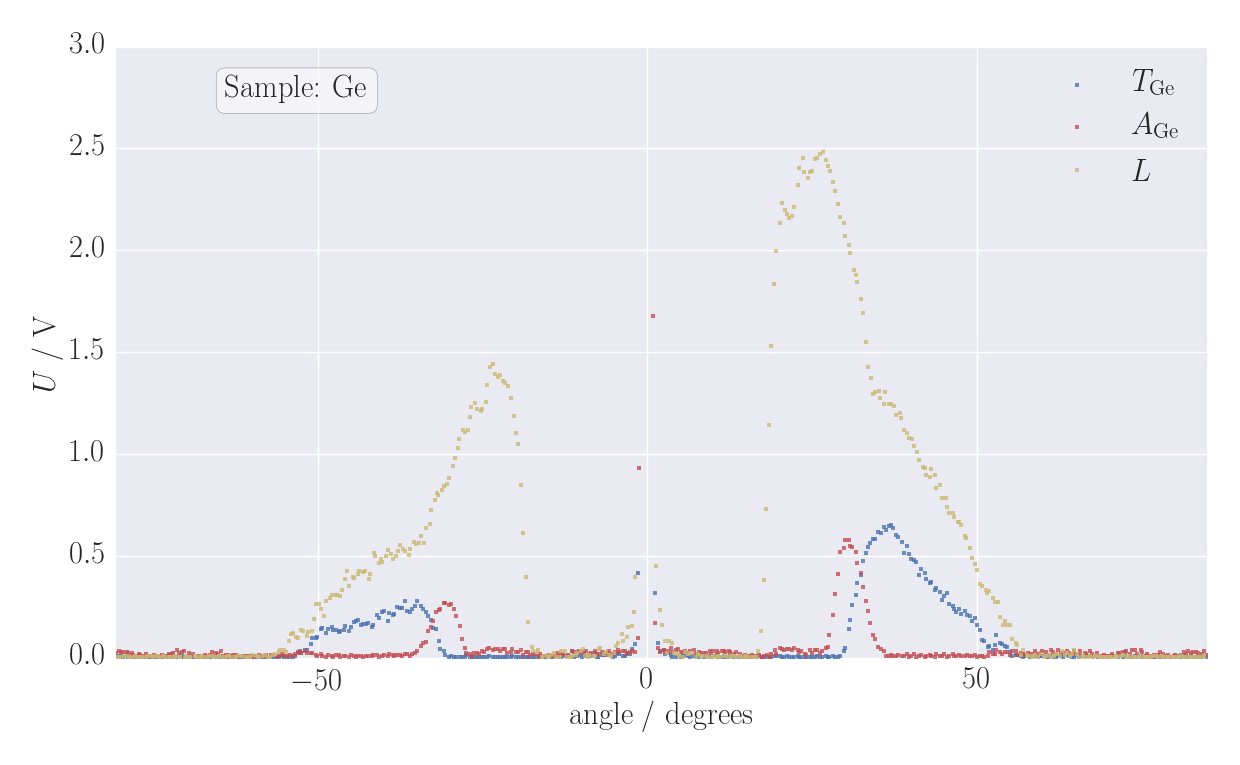
\includegraphics[width=1.0\linewidth]{figures/band_gap_raw_Ge}
        \caption{}
        \label{fig:band_gap_raw_Ge}
    \end{subfigure}
    \begin{subfigure}[b]{\pltw}
        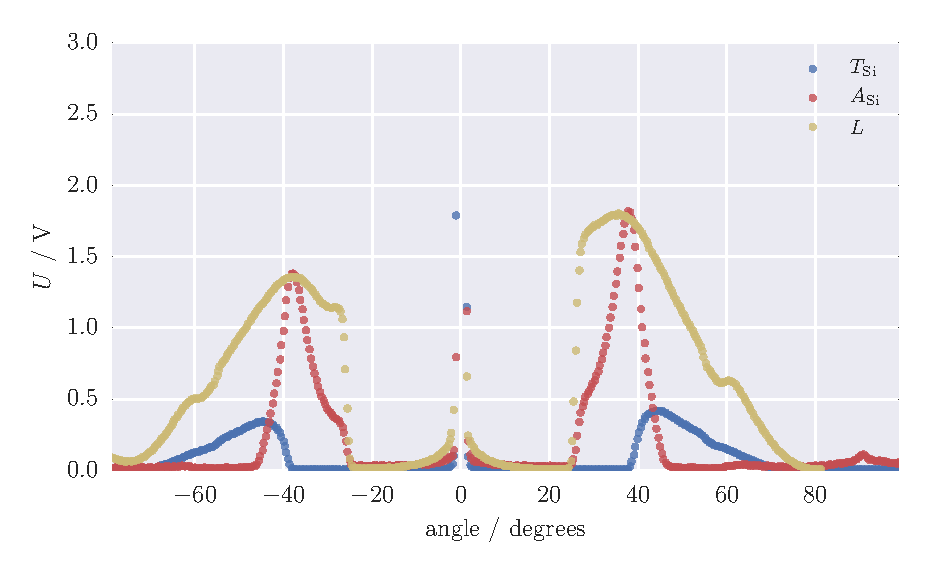
\includegraphics[width=1.0\linewidth]{figures/band_gap_raw_Si}
        \caption{}
        \label{fig:band_gap_raw_Si}
    \end{subfigure}
    \caption{
        The signals measured with Ge (\ref{fig:band_gap_raw_Ge}) 
        and Si (\ref{fig:band_gap_raw_Si}) as samples with corresponding 
        grating and filter. $T$ and $A$ indicate 
        the transmission and absorption, measured by the currents through 
        the pyrodetector and the semiconductor, respectively. 
        $L$ is the intensity of the lamp with installed filter, measured 
        without the semiconductor. The asymmetry might be due to 
        irregularities on the grating or within the beam path. 
        }
    \label{fig:band_gap}
\end{figure}

The evaluation for both samples is done 
absolutely analogously. We thus explain the steps for the example 
of Ge plotting all necessary steps, while the plots for 
Si are added to the appendix, \ref{sec:appendix_band_gap_plots}.
In order to apply the formulas \eqref{eq:t_real} and \eqref{eq:a_real}
for the real transmission and absorption, we had to interpolate the data, 
because the angles measured for all three quantities involved did 
non agree. From each data set, e.~g. angles $\phi$ and measured transmission $T$ 
and absorption $A$ with the Ge sample installed, we created a traverse function 
interpolating $T$ and $A$ on a predefined grid. 
Calculating $T$ at angle $\phi$ was done in the following manner:
Let $(\phi_1, T_1)$ and 
$(\phi_2, T_2)$ be the pairs of data with $\phi_1$ and $\phi_2$ the 
next angles on the left and right of $\phi$, respectively. 
Then, 
\begin{equation}
    T = \frac{1}{(\phi_2 - \phi_1)} 
        \left(T_1\left(\phi - \phi_1\right) + T_2\left(\phi_2 - \phi\right)\right)
\end{equation}

The result of this procedure can be seen in figure~\ref{fig:band_gap_detail_Ge_left}, 
showing a detail of the entire spectrum on the left side ($\phi < 0^\circ$). 
This figure will not be shown for the other side or the Si sample, as 
it has only exemplary character. 
Seeking the intersect of the straight lines interpolated at the transition from 
absorption to transmission is done on yet a smaller scale. Here, 
the signals are normalized, setting $T = 1$ and $A = 1$ for the according maxima, 
when the antagonist is close to zero. The fit is then done choosing the 
points which are used manually. The results together with the points chosen for fitting 
are displayed in figure~\ref{fig:band_gap_result_Ge_left}. 
\begin{figure}
    \centering
    \begin{subfigure}[b]{\pltw}
        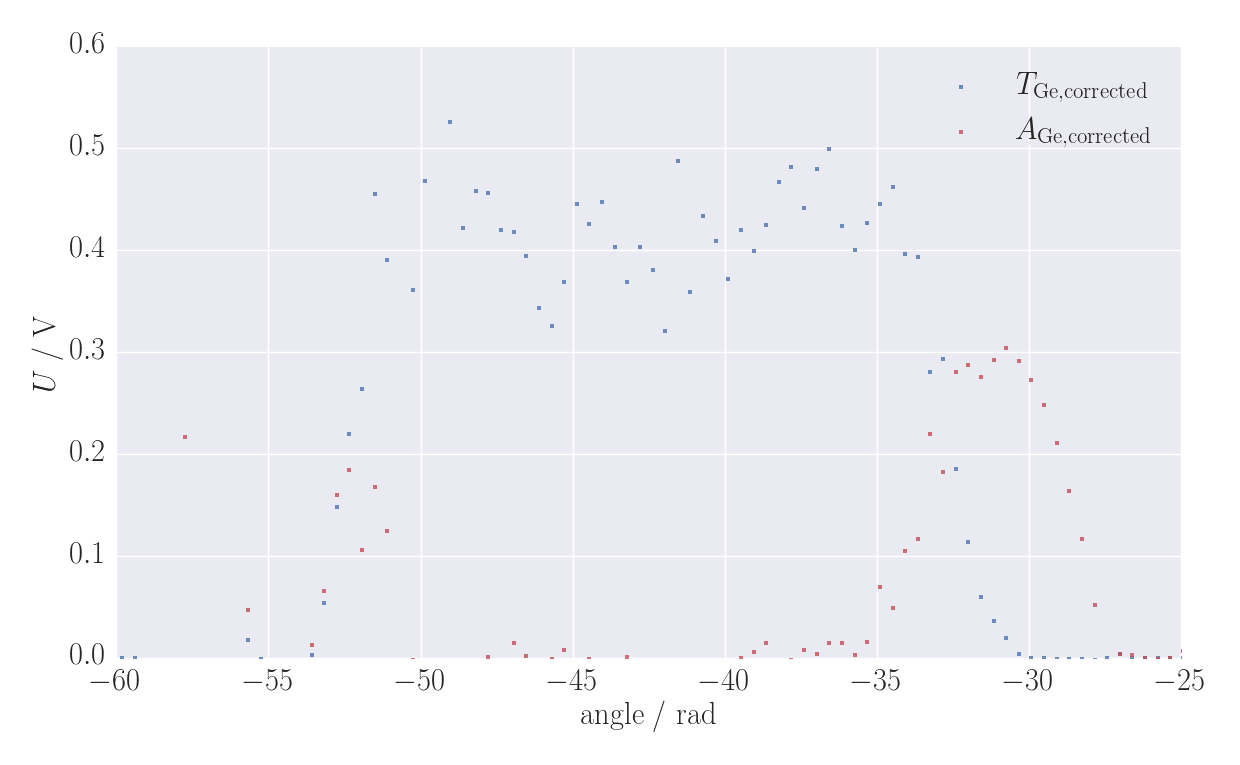
\includegraphics[width=1.0\linewidth]{figures/band_gap_detail_Ge_left}
        \caption{
            Detail of the transmission and absorption, corrected for the 
            background and the spectrum of the lamp. The region we are interested 
            in for further evaluation if the intersect of $T$ and $A$ in
            the right half of the plot. 
            }
        \label{fig:band_gap_detail_Ge_left}
    \end{subfigure}
    \begin{subfigure}[b]{\pltw}
        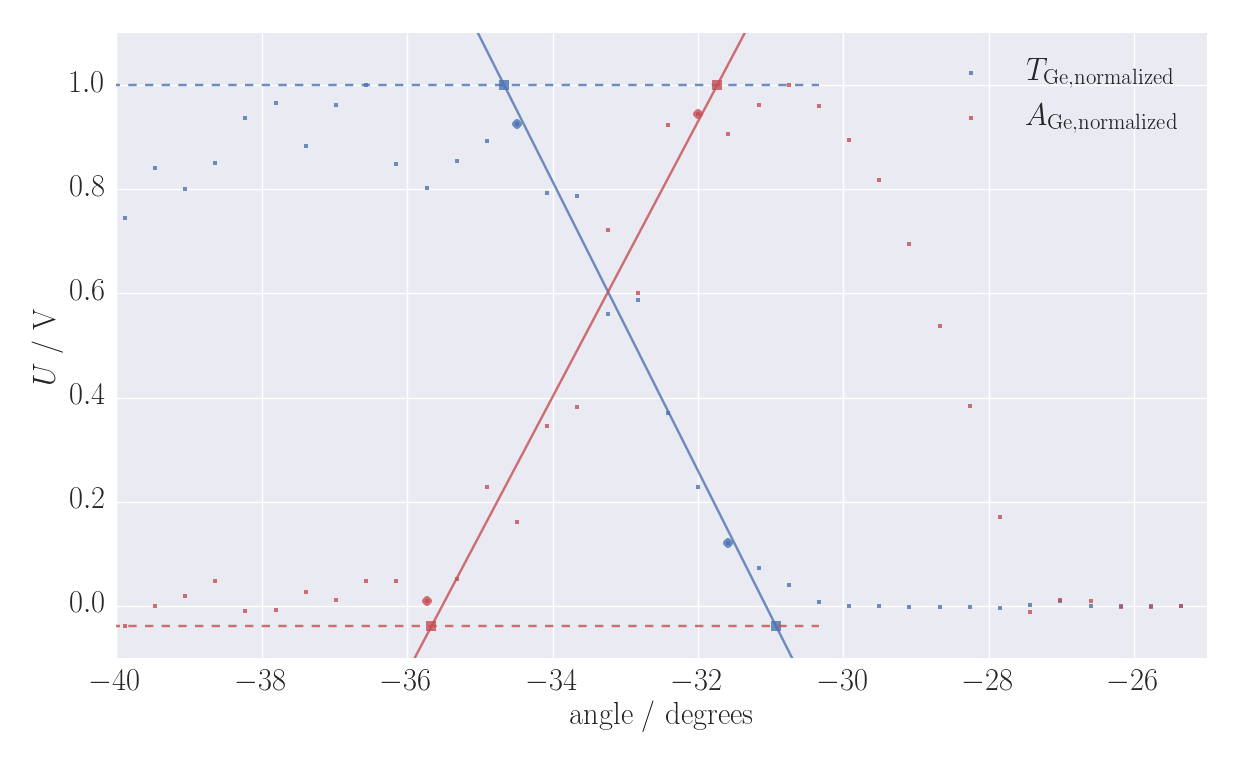
\includegraphics[width=1.0\linewidth]{figures/band_gap_result_Ge_left}
        \caption{
            Result of the procedure fitting straight lines through the points 
            at the transition from transmitting to absorbing characteristic. 
            The larger round dots indicate the upper and lower limit 
            chosen for the interpolation. The dashed line corresponds to 
            the maximum of transmission and minimum of absorption, the 
            squares to the respective intersects with the straight lines.
            In order to maintain clarity, 
            the values for the angles at the intersects are given in the text. 
            The nominal value for the band gap energy is given by the intersect 
            of the two lines. 
            }
        \label{fig:band_gap_result_Ge_left}
    \end{subfigure}
    \caption{
        Plots corresponding to the calculation of $\alpha_g$ which is then be 
        used to calculate the band gap energy $E_g$. 
        }
    \label{fig:band_gap_result_Ge}
\end{figure}
The band gap energy is thus reached for an angle of $\phi_g = 123^\circ$, 
which applying equation~\eqref{eq:E_g} yields:
\begin{equation}
    E_g = 123
\end{equation}
One can observe BLABLABLABLABL

For the right side, the respective plot is shown in the appendix, 
figure~\ref{fig:band_gap_result_Ge_right}, followed by those for the 
silicon (\ref{fig:band_gap_result_Si_left}, \ref{fig:band_gap_result_Si_right}). 
The results are displayed in table \ref{tab:band_gap_results}.
